\documentclass[a4paper,12pt,twocolumn]{report}
\usepackage[utf8]{inputenc}
\usepackage{graphicx}
\usepackage{natbib}   % omit 'round' option if you prefer square brackets
\graphicspath{ {img/} }


% Title Page
\title{CM30229 - Room Circumnavigation using LEJOS}
\author{Dominic Hauton}


\begin{document}
\maketitle
\bibliographystyle{plainnat}
\begin{abstract}
\end{abstract}

\section{Introduction}
% All of your courseworks are designed primarily to give you experience in developing intelligent control and/or cognitive systems. However, the course is also intended to give you experience and feedback in writing about research. To this end, you will be writing research reports of about two pages, using exactly this format.

% The Introduction of a research report should give a brief description of what you you tried to do (your hypothesis), and the outcome. It should also give some idea about why you have done it (motivation). In doing this, you may also give a brief background argument. I expect you to cite a paper or two for this motivational context. For coursework 1, one of the papers you should probably cite is Brooks (1991), since you have been asked to take a fairly reactive approach to developing robot intelligence.

% Coursework one requires you to construct a robot capable of circumnavigating rooms or other closed spaces (don’t worry about doorways – just close or block them.) Ideally this should work in “natural” (unaltered) indoor environments with a variety of obstacles along the walls, but often people build up some barriers. However, the report should not be about the entire experience of building a robot, but rather it should present a single hypothesis you tested on your completed robot about how to improve its intelligence.

The goal of this research is to see the effect of sensor loop times on the navigation capabilities of the rover while circumnavigating a room. The rover was built using parts from the LEGO Mindstorm NXJ kit. There were 3 sensors; a \emph{Sonar}, \emph{Light Sensor} and \emph{Bump Sensor} (x3). Three motors were provided for movement and navigation.

To make informed decisions all of the sensors were used and the sonar was mounted on a pivot to allow for measurements in multiple directions, as shown in figure \ref{fig:stanley-head}. To provide movement two driven wheels were used and a trolley wheel was placed at the back for stability.

\begin{figure}[b]
 \includegraphics[width=0.5\textwidth]{headshot}
 \caption{Rover Head Sensor}
 \label{fig:stanley-head}
\end{figure}

During development a reactive approach was taken, using the subsumption architecture \citep{wooldridge2009introduction} with emphasis on sensing using multiple layers of perception to allow for informed movement decisions. The use of the subsumption architecture was based on Brooks' theses that Intelligence is an emergent property of certain complex systems. \citep{brooks1991intelligence} During development this subsumption approach was added into the perception mechanism, during which the rover had to to decide on it's current situation.

\section{Approach}

% The approach describes in detail exactly what you have done. This section is longer, and should ideally include some experiments you set up, for example to determine in what conditions you could get better results from the robot. The approach should be in sufficient detail that another person could replicate your experiments. You may cite other papers here too if you are taking an approach from another paper, or modifying it only slightly.

% Please do mention who shared your robot in the approach section, and the extent to which you worked together. The objective here is to learn. How much you work together is totally up to you so long as you each write your report independently.

% Submissions should be in PDF or HTML, preferably derived from this latex format, certainly in 12 point font. I recommend making HTML by using latex plus htlatex, but you can construct your report using any tool you please. Note that this specification is exactly 2 pages long, so an HTML report should be no longer than this. Figures (both drawn plans and photos) are encouraged for marks and clarity and do not count either for or against page length. The 1–2 pages are counting text only (not citations). But remember, don’t spend too much time on this coursework! You should spend about 19 hours total on each coursework, about 4 of which will be writing up. The coursework should be uploaded to Moodle by 11pm on Friday 3 March at the latest, but feel free to submit it (much) sooner.

% To quantify the outcomes of this coursework, you may want to think about questions such as contrasting the addition of extra control algorithms, changing the physical shape of the robot, or trying different target sonar readings for maintaining a particular distance from the wall in a variety of contexts. These can be quantified in terms of the circuit time for the robot, the success rate, or any other metric you can think of.

% For coursework one, it is quite likely that you will not have initially thought of a hypothesis to test, but will rather just have tried to make the robot work. However, in your exploration (both with the robot and with your reading) you should always be looking to something that seems to make a difference in performance, and then try to capture what that something is. Can you describe it ex you get given how much change you make to some parameter on the robot? Don’t forget to consider things such as the battery charge, operating in daylight, or proximity to other sonar-using robots as possible explanations for strange behaviour.

The initial design of the rover was a simple reflex agent as described by \cite{russell1995modern}. This took the sensor readings, and using transduction converted them to a proximity reading in every direction. This allowed to rover to react to a crash but when recovering from a crash the rover had no context. As a result I settled on \cite{russell1995modern}'s model-based reflex agent. This allows the sensors to modify the state at individual rates, in the final design there were two sensing thread loops, operating at different tick rates, as shown in figure \ref{fig:perception}. One for the sonar which provided slow but accurate readings and one for the other sensors which provided almost instantaneous measurements.

All of the sensor readings were mixed and the closest reading was taken. This was especially important for the front sensor where 3 separate readings were taken from the bump, light and sonar sensor. To improve sensor quality 15 readings were taken every measurement and any reading more than two standard deviations away from the mean were thrown out, and the remainder of the readings were averaged.

\begin{figure}
 \includegraphics[width=0.5\textwidth]{sensing-diagram}
 \caption{Final Perception Architecture}
 \label{fig:perception}
\end{figure}

Throughout the research the rover was shared with Ryan Cullen. In the first part of the coursework the rover resided in my house. I built the rover itself, optimising it's design over several iterations and created the perception system of the code. The software continuously modified proximity readings in the state, indicating how close the rover was to an object in all four cardinal directions. At this point the code was then forked by Ryan and we each developed our own action selection code based on the rover state.

\begin{figure}[b]
 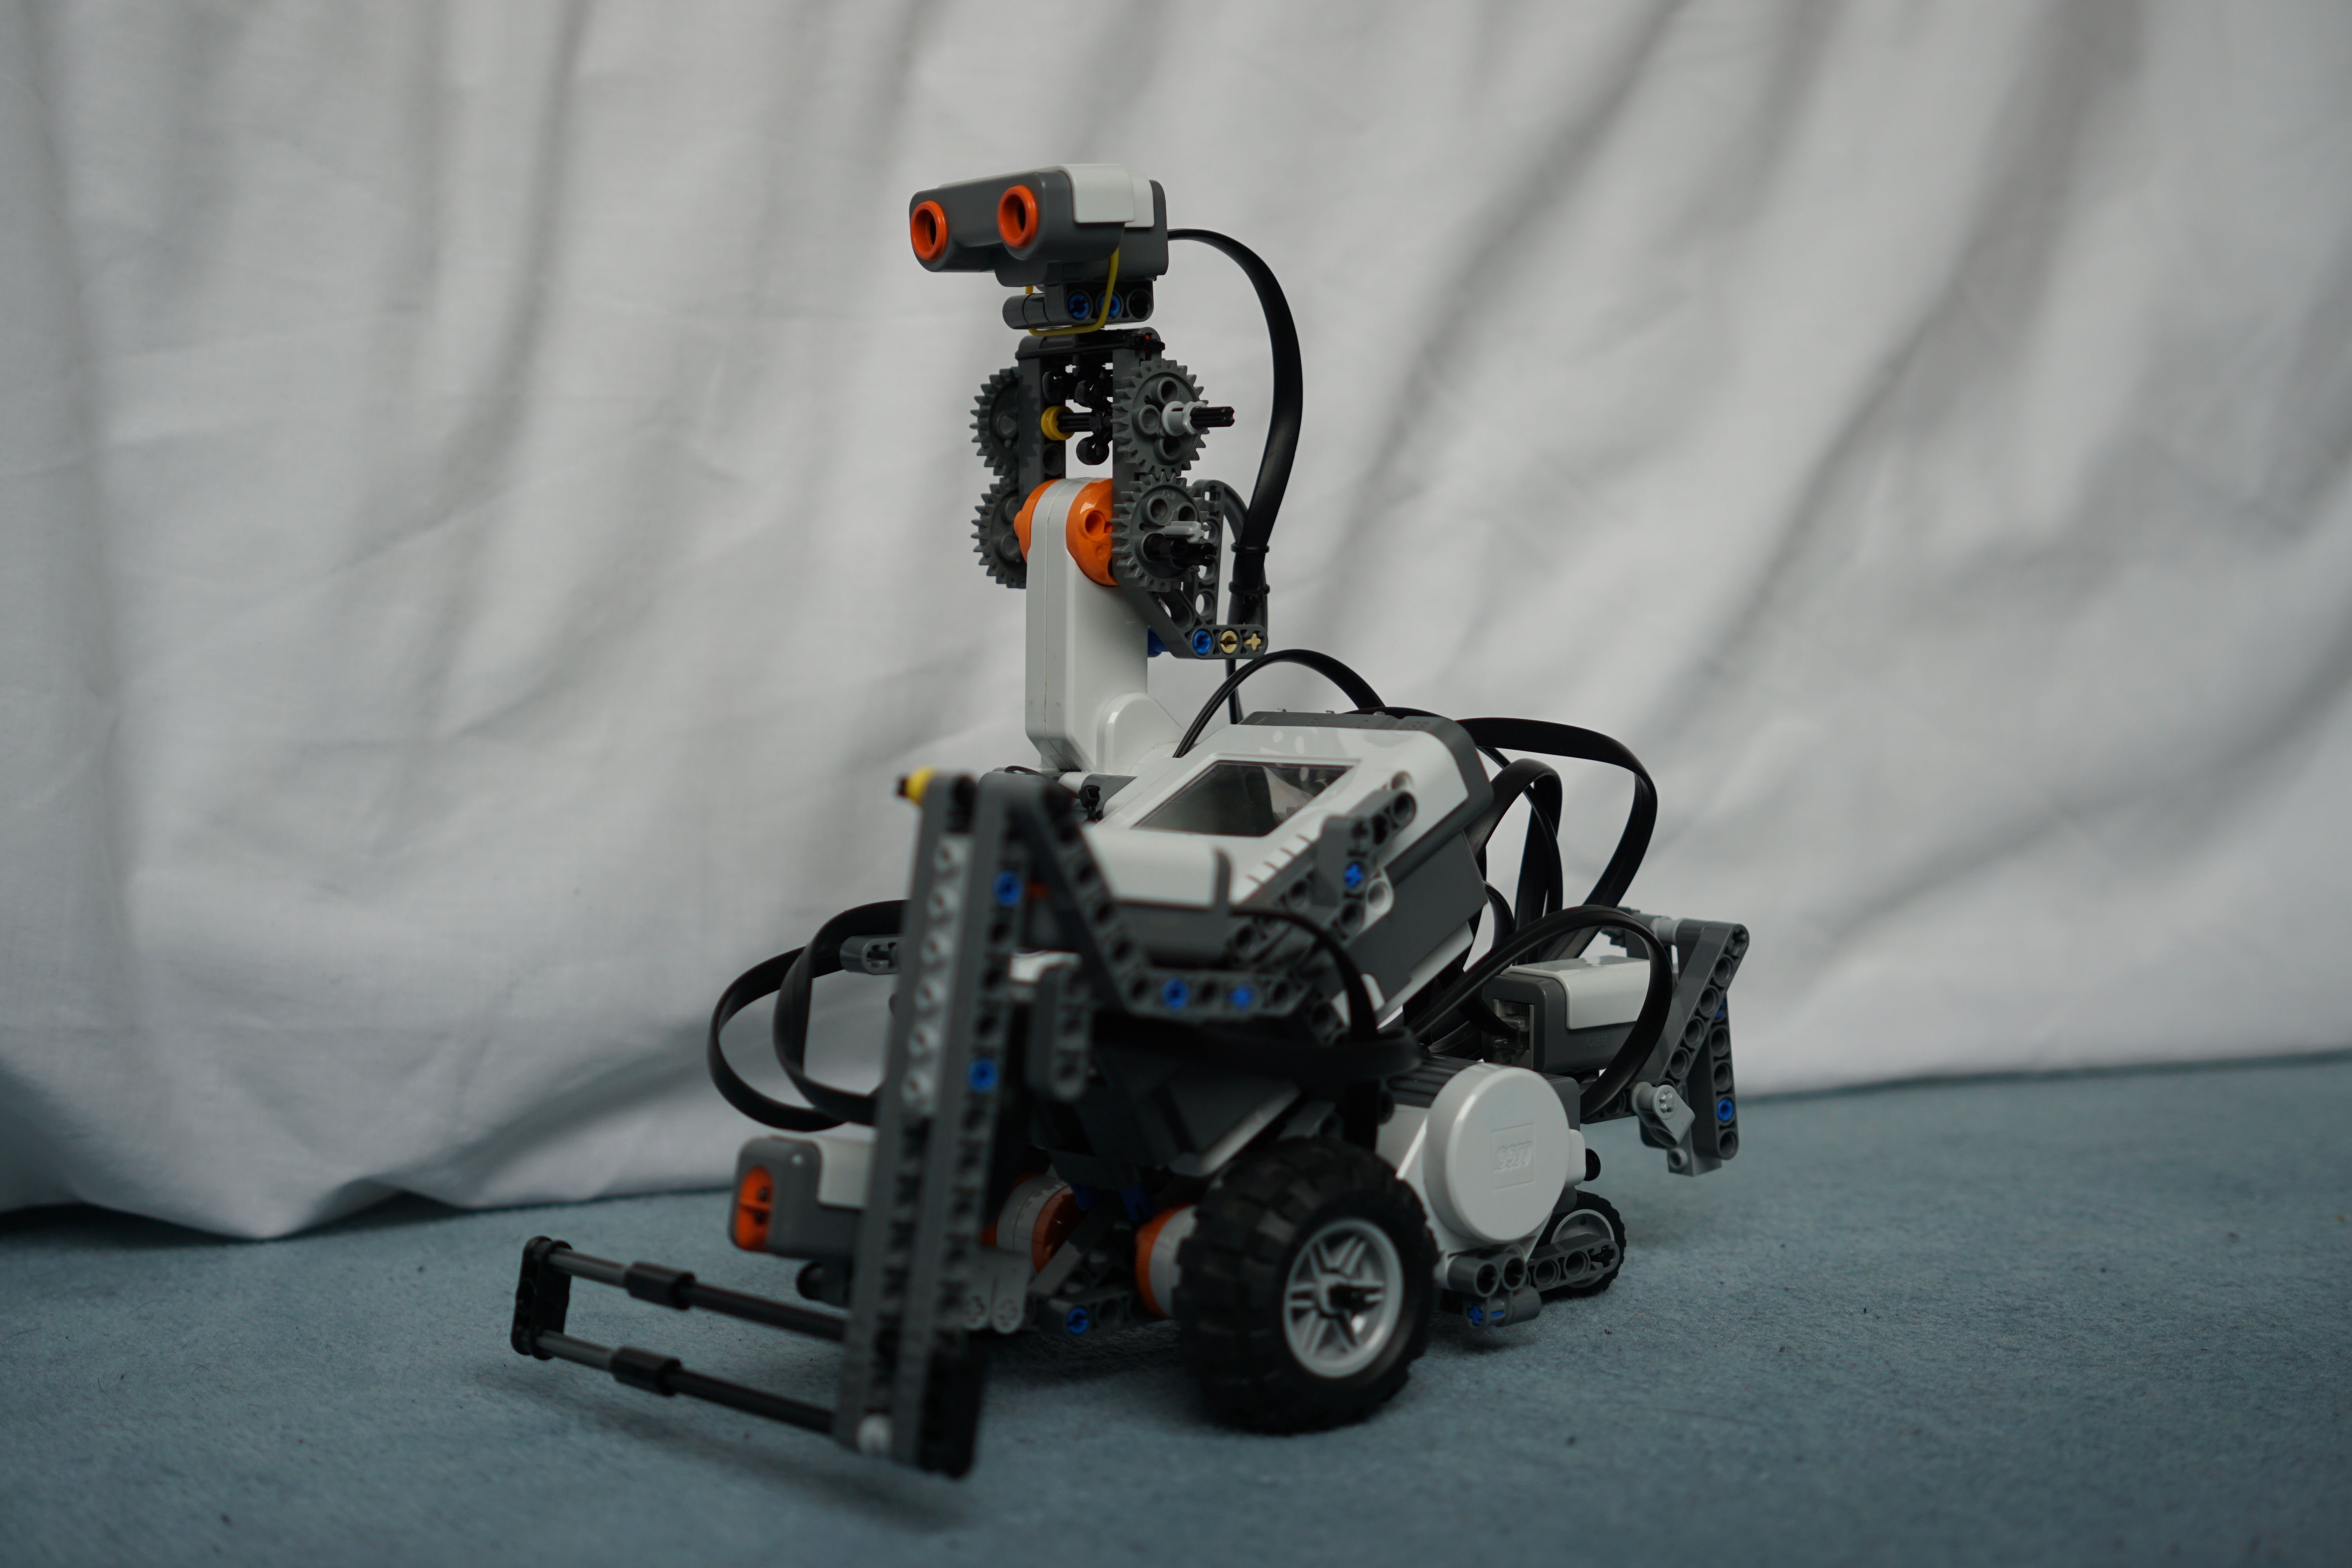
\includegraphics[width=0.5\textwidth]{full}
 \caption{Stanley Rover}
 \label{fig:stanley}
\end{figure}

\section{Results}

% The results section describes the outcomes. This should be purely factual descriptions, including qualitative outcomes, quantitative outcomes and possibly statistics. For example, you could report the average speed around a circuit in two conditions plus standard deviations and a significance test to tell whether you have evidence that the conditions lead to different results. For coursework 1, this must include video. Typically, the results section can be surprisingly short, since the Approach section is the one giving details. Results are purely and only factual outcomes (no alternative facts).

% With respect to your personal results, if you describe a reasonably-well working system in a comprehensible manner you will pass. If you competently fill in all of these sections as described in this specification, you will get at least 55. Getting a mark over 70 requires demonstrating insight, creativity and / or understanding that goes beyond the basics laid out for you in this document. For example, an insightful comment about one or more cited papers supported by evidence from your experience might get you these extra marks. So might a particularly accurate and replicable account of your approach and results.

% https://www.youtube.com/watch?v=LOPdO0w1Uec

\section{Discussion}

% The discussion is the most discursive part of your paper, it may include speculation. You should discuss the extent to which your results addressed the questions described in your introduction, and what the results imply about your own work and AI or robotics more broadly. You might suggest other experimental protocols that could have given different results and lessons learned. This can be a longer section, and may again include citations if you compare or contrast to other published accounts.

\section{Conclusion}

% The conclusion is just one paragraph. After possible digressions in the discussion, you should come back to restate exactly what you tried to do (brief summary of the introduction), what the outcome was (brief summary of the results), and what you can certainly state as a result of this (the implications of the results in light of the introduction.)

\bibliography{lejos-writeup}

\end{document}
